\documentclass[11pt,a4paper]{article}

\usepackage[utf8]{inputenc}
\usepackage[T1]{fontenc}
\usepackage[spanish]{babel}
\usepackage{lmodern}
\usepackage[a4paper,margin=2.5cm]{geometry}
\usepackage{graphicx}
\usepackage{booktabs}
\usepackage{amsmath}
\usepackage{enumitem}
\usepackage[hidelinks]{hyperref}

\setlength{\parindent}{0pt}
\setlength{\parskip}{0.7em}
\emergencystretch=3em

% Nombre de un campo o archivo de los datos (admite guiones bajos).
\newcommand{\campo}[1]{\texttt{\detokenize{#1}}}

\begin{document}

% ---------------------------------------------------------------- Portada
\begin{titlepage}
  \centering
  
\includegraphics[height=2.6cm]{logo-informatica.png}
  \hfill
  
\includegraphics[height=2.6cm]{logo-uncoma.png}

  \vspace{2.2cm}
  {\large Departamento Teoría de la Computación\par}
  {\large\textbf{Facultad de Informática}\par}
  {\large Universidad Nacional del Comahue\par}

  \vspace{1.8cm}
  {\huge Laboratorio de inteligencia artificial\par}
  \vspace{0.4cm}
  {\Large Trabajo Práctico Obligatorio N\textsuperscript{o} 1\par}
  \vspace{0.3cm}
  \vspace{0.5cm}
  {\LARGE\textbf{Exploración y corpus}\par}
  \vspace{0.2cm}
  {\normalsize Predicción de la duración de desvíos de ruta en flotas de transporte de personal\par}

  \vspace{1.2cm}
  \begin{tabular}{@{}lll@{}}
    \toprule
    \textbf{Apellido y Nombre} & \textbf{Legajo} & \textbf{Email} \\
    \midrule
    Reibold, Sebastian Alejandro & FAI-3854 & sebastian.reibold@est.fi.uncoma.edu.ar \\
    Fernandez Gramajo, Bautista  & FAI-3874 & bautista.fernandez@est.fi.uncoma.edu.ar \\
    Kissner, Davor               & FAI-3185 & davor.kissner@est.fi.uncoma.edu.ar \\
    \bottomrule
  \end{tabular}

  \vfill
  {\large Cursado 2026 \quad---\quad 29 de octubre de 2026\par}
\end{titlepage}

% ---------------------------------------------------------------- Índice
\tableofcontents
\newpage

% ---------------------------------------------------------------- 1
\section{Introducción}

Este documento presenta la exploración de los datos de Tecfield y la construcción del corpus de
trabajo del proyecto, que busca estimar, en el instante en que aparece el primer punto fuera de ruta
de un vehículo ($T_0$), cuánto va a durar el desvío. Los números provienen de la ejecución completa
del cuaderno de Python \campo{notebooks/01_exploracion_y_modelos.py}, sobre las tres
colecciones que entregó la empresa.

El documento se organiza así: la sección~2 describe y caracteriza cada colección y los problemas de
calidad encontrados; la sección~3 explica cómo se arma el corpus, con una fila por evento de desvío;
la sección~4 presenta los modelos planteados para probar sobre ese corpus; y la sección~5 cierra con
los pasos siguientes.

% ---------------------------------------------------------------- 2
\section{Exploración de los datos}

\subsection{Las tres colecciones}

Tecfield proveyó tres colecciones exportadas de MongoDB (Extended JSON, un documento por línea), que
suman unos 1,9 GB. Las fechas vienen en UTC y se pasan a hora de Argentina (UTC$-$3) antes de agrupar
por día.

\begin{table}[h]
  \centering
  \begin{tabular}{@{}lrrll@{}}
    \toprule
    \textbf{Colección} & \textbf{Filas} & \textbf{Vehículos} & \textbf{Período} & \textbf{Qué contiene} \\
    \midrule
    \campo{hojaDeRuta}      & 5.519     & 584 & 22/10/2025 -- 09/09/2026 & plan del viaje \\
    \campo{desviosHojaRuta} & 203.897   & 584 & 09/06/2026 -- 31/08/2026 & puntos fuera de ruta \\
    \campo{rastreoSatelital} & 1.683.550 & 583 & 12/07/2026 -- 31/08/2026 & eventos del GPS \\
    \bottomrule
  \end{tabular}
  \caption{Tamaño y período de cada colección. En hojas de ruta el período es el de vigencia
  (\campo{fechaDesde}--\campo{fechaHasta}); en las otras dos, el de las fechas del GPS.}
\end{table}

Hay tres rarezas de formato que condicionan todo el procesamiento. El vehículo se llama
\campo{vehiculo.id} en hojas de ruta, \campo{flotaId} en desvíos y \campo{flotaID} en rastreo. Las
coordenadas son \texttt{[lat, lon]} en desvíos y en la ruta planificada, pero \texttt{[lon, lat]} en
rastreo. Y el trazado de la ruta de cada hoja (calculado con OSRM, un servicio de mapas) pesa el
99\,\% del archivo de 1,5 GB, así que se descarta al cargar y solo se conservan los datos simples y los conteos.

\subsection{Hojas de ruta}

Cada hoja asigna a un vehículo un recorrido planificado hacia una obra. De las 5.519 hojas, 5.013 están
vencidas y 506 vigentes; corresponden a 62 obras distintas. El tipo de vehículo más frecuente es
\emph{Pesada} (2.900 hojas), seguido de \emph{Liviana} (996) y \emph{Rutero} (515). El campo
\campo{tipoHDR} es nulo en 2.674 hojas; el resto se reparte entre transporte de personal (1.363),
registro de transporte (1.240) y gerenciamiento de viaje (242).

El recorrido de ida mide en promedio 114 km y 112 minutos según OSRM, con 4,2 paradas y 5,2
puntos de paso por hoja. Las hojas llevan en promedio 6,0 pasajeros para 8,0 plazas; entre las 1.560
hojas con plazas informadas la ocupación media es del 66\,\%, y el 54\,\% de todas las hojas no tiene
ningún pasajero.

\subsection{Desvíos}

La colección contiene 203.897 puntos fuera de ruta, agrupados por \campo{grupoDesvioId} en 37.720
episodios, de 584 vehículos y 5.523 hojas de ruta distintas. El detector registró el retorno por
ubicación en 130.319 puntos y por \emph{timeout} en 68.014 (5.564 sin motivo). La ruta más cercana al
punto es la de ida en el 67\,\% de los casos, la de vuelta en el 19\,\% y la alternativa en el 14\,\%.
La velocidad es nula en el 28\,\% de los puntos y \campo{tipoHDR} está presente solo en el 45\,\%.

Un hallazgo importante es la demora entre el instante en que el GPS midió la posición
(\campo{fechaHoraRastreo}) y el momento en que se registró el punto de desvío (\campo{timestamp}). La
mediana es de 1 minuto y el percentil 95 de 20, pero el percentil 99 llega a 1.283 minutos y el máximo
a 98.698. En 6.768 puntos (3,3\,\%) la posición GPS tiene más de una hora de antigüedad. Por eso la
duración se mide con la hora del GPS y no con la de registro.

En una primera aproximación por episodio (midiendo con la hora de registro), la duración mediana es de
10 minutos, con cuartiles de 4 y 49, pero la media supera las 4 horas (257 minutos): la distribución
tiene una cola muy larga. Los episodios tienen una mediana de 3 puntos, y la distancia máxima a la ruta
tiene mediana de 4,8 km.

\subsection{Rastreo satelital}

Son 1.683.550 eventos de 583 vehículos y 113 tipos de evento (posición programada, vehículo detenido,
excesos de velocidad, entre otros). El 8\,\% de las filas (129.634) está exactamente duplicado. De los
4.308 eventos de ``límite de velocidad superado'', el 10\,\% informa velocidad igual a cero, lo que
vuelve poco confiable ese campo. La velocidad mediana es 0 y la máxima 280 km/h. Hay 2.809 eventos
fuera de la Argentina o sin coordenadas.

\subsection{Cruce entre colecciones}

El vehículo es lo único que une las tres colecciones y además cada desvío apunta a su hoja con
\campo{hojaDeRutaId}. La cobertura es casi completa: los 584 vehículos con desvíos tienen hoja de ruta,
583 de ellos aparecen en el rastreo, y los 583 vehículos del rastreo tienen hoja. Solo 4 de los 5.523
identificadores de hoja citados en desvíos no existen en \campo{hojaDeRuta} (79 puntos). Entre desvíos
y rastreo no hay un identificador común: hay que cruzar por vehículo y hora.

Aparecen dos problemas de calidad que afectan al corpus:

\begin{itemize}[nosep]
  \item \textbf{Hojas vencidas.} El 61\,\% de los puntos (124.588) cae fuera de la vigencia de su hoja
  de ruta: 792 antes de \campo{fechaDesde} y 123.796 después de \campo{fechaHasta}, con una mediana de
  27 días fuera (percentil 90: 88; máximo: 279). Parece que el sistema sigue comparando contra hojas
  ya vencidas. Solo 3.617 de las 5.519 hojas estaban vigentes durante la ventana del rastreo.
  \item \textbf{Puntos repetidos.} Los 203.897 puntos corresponden a solo 120.943 posiciones GPS
  distintas (vehículo más hora): un mismo punto se guarda contra varias hojas de ruta, de modo que
  un mismo desvío puede aparecer repetido.
\end{itemize}

También hay que notar que el rastreo comienza el 12/07/2026 y los desvíos el 09/06/2026, por lo que
los desvíos anteriores a esa fecha no pueden tener rastreo previo a $T_0$.

% ---------------------------------------------------------------- 3
\section{Construcción del corpus}

\subsection{Unidad de análisis y variable objetivo}

La unidad de análisis es el \emph{evento}, es decir, un \campo{grupoDesvioId}, y no la lectura. El
instante $T_0$ es el primer \campo{fechaHoraRastreo} del evento, y la variable objetivo $y$ es la
diferencia, en segundos, entre el último y el primer \campo{fechaHoraRastreo}. El evento cierra cuando
el vehículo retoma la ruta o cuando el detector alcanza su tope de cuatro horas.

\subsection{Reglas de armado}

\begin{enumerate}[nosep]
  \item Se descartan las lecturas con posición $(0,0)$ (un GPS sin señal) o con fecha fuera de
  2025--2026.
  \item Se agrupan las lecturas válidas por \campo{grupoDesvioId}: del primer ping salen los atributos
  de $T_0$ (ordenado por hora del GPS, y por distancia y posición para desempatar), y de todo el
  grupo salen la cantidad de lecturas y la duración $y$.
  \item Se agregan los datos de la hoja de ruta correspondiente y se calcula si estaba vigente en
  $T_0$.
  \item Cuando un mismo desvío se guardó contra varias hojas, se deja un solo evento por vehículo y
  $T_0$, prefiriendo el de la hoja vigente.
  \item Se calcula el comportamiento del vehículo en los 10 minutos anteriores a $T_0$ (sin incluir
  $T_0$) con una búsqueda del último y del primer GPS de la ventana.
  \item Se entrena solo con eventos de dos o más lecturas y duración mayor a cero. Los que llegan al
  tope de cuatro horas se separan: no corresponden a un retorno medido.
\end{enumerate}

Solo se usa información disponible en $T_0$. Quedan afuera los campos de retorno, la cantidad de
lecturas del evento y todo lo posterior a $T_0$, para que el modelo no use información del futuro.

\subsection{Atributos en $T_0$}

Se definieron 23 atributos en tres grupos, según su origen.

\begin{table}[h]
  \centering
  \begin{tabular}{@{}lp{10.5cm}@{}}
    \toprule
    \textbf{Grupo} & \textbf{Atributos} \\
    \midrule
    Primer ping &
      distancia a la ruta, velocidad y si viene vacía, ruta más cercana (ida, vuelta o alternativa),
      latitud, longitud, hora, día de la semana y franja (madrugada, mañana, tarde, noche) \\
    Hoja de ruta &
      tipo de vehículo, tipo de hoja, obra, largo y duración estimada de la ida, plazas, pasajeros y si la
      hoja estaba vigente en $T_0$ \\
    Rastreo previo &
      cantidad de GPS, velocidad media y última, minutos desde el último GPS, desplazamiento en línea
      recta y rumbo, todo en los 10 minutos previos a $T_0$ \\
    \bottomrule
  \end{tabular}
  \caption{Atributos conocidos en $T_0$.}
\end{table}

\subsection{El corpus resultante}

\begin{table}[h]
  \centering
  \begin{tabular}{@{}lr@{}}
    \toprule
    \textbf{Paso} & \textbf{Eventos} \\
    \midrule
    Eventos con lecturas válidas                       & 37.720 \\
    Repetidos contra otra hoja (mismo vehículo y $T_0$) & 2.007 \\
    Una sola lectura o duración cero (se descartan)    & 19.240 \\
    Llegan al tope de 4 h (aparte, sin retorno medido) & 2.841 \\
    \midrule
    \textbf{Corpus para entrenar}                      & \textbf{13.632} \\
    \bottomrule
  \end{tabular}
  \caption{De los eventos a los datos de entrenamiento. El corpus final cubre 556 vehículos.}
\end{table}

La duración en el corpus tiene mediana de 20,4 minutos y percentil 90 de 115,8 minutos (cuartiles de
10 y 53 minutos). La figura~\ref{fig:hist} muestra la distribución, con la cola hacia el tope de cuatro
horas.

\begin{figure}[h]
  \centering
  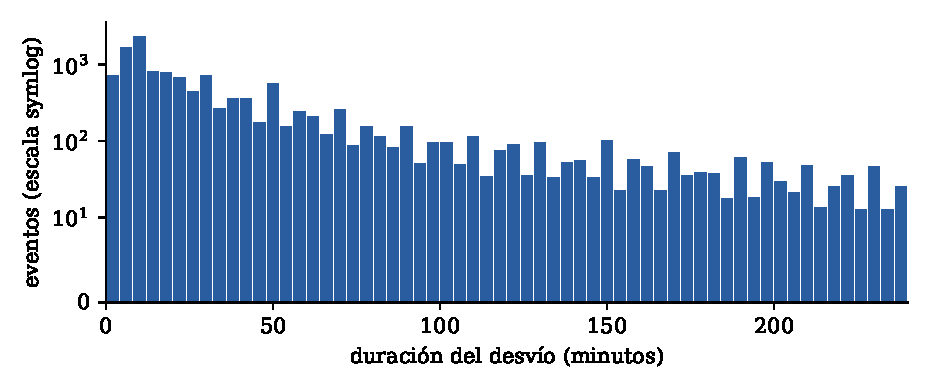
\includegraphics[width=0.85\textwidth]{fig-histograma.pdf}
  \caption{Duración de los desvíos del corpus, en barras de 4 minutos.}
  \label{fig:hist}
\end{figure}

La cobertura de los atributos es desigual. Solo 7.854 de los 13.632 eventos (58\,\%) tienen algún GPS
en los 10 minutos previos, y para solo 1.838 hay rumbo (hacen falta dos o más puntos). La velocidad del
primer ping falta en 2.247 eventos y 6.804 no tienen \campo{tipoHDR}. El 99,99\,\% de los eventos
tiene hoja de ruta asociada.

% ---------------------------------------------------------------- 4
\section{Modelos planteados}

Con el corpus armado, se plantea comparar tres formas de predecir la duración de un desvío. Todavía
no se probaron: esta sección define qué se va a probar y cómo se va a medir.

\subsection{Qué se compara}

\begin{itemize}[nosep]
  \item \textbf{Referencia:} predecir siempre la misma duración, la mediana de los desvíos de
  entrenamiento. Es lo mínimo que un modelo tiene que superar.
  \item \textbf{Árbol de decisión:} hace una serie de preguntas sobre el desvío (por ejemplo, si la
  distancia a la ruta supera cierto valor o si es de noche) y termina en una duración estimada. Se
  limita su tamaño para que no memorice los casos.
  \item \textbf{Bosque aleatorio (\emph{Random Forest}):} promedia las respuestas de 200 árboles de
  decisión distintos.
  \item \textbf{Refuerzo de gradiente (\emph{gradient boosting}):} arma árboles de a uno, y cada uno
  corrige los errores de los anteriores.
\end{itemize}

Los tres aprenderían la duración en escala logarítmica, $\log(1+y)$, porque hay muchos desvíos cortos
y pocos muy largos; así los largos no dominan el aprendizaje, como sugiere el enfoque de modelos de
duración de Hojati et al.~\cite{hojati}.

\subsection{Cómo se mide}

Para saber si un modelo sirve, se lo prueba con vehículos que no vio al entrenar. Los vehículos se
reparten en cinco grupos y cada grupo se usa una vez como prueba, mientras los otros cuatro sirven de
entrenamiento (validación cruzada por vehículo). Konovalenko et al.~\cite{konovalenko} separan los datos
por fecha; acá se separa por vehículo para que el modelo no memorice cómo se comporta cada móvil.

El error se mide en minutos con dos números: el error promedio (la diferencia absoluta media entre la
duración predicha y la real, conocido como MAE) y el error mediano. Además se calcula en qué porcentaje
mejora el error promedio respecto de la referencia.

\subsection{Selección de atributos}

Los 23 atributos del cuadro~2 se pueden quitar o agregar para ver si con menos ya alcanza. Se plantea
sumar los grupos de a uno (primer ping, hoja de ruta, rastreo previo) y medir el error cada vez, para
saber cuánto aporta cada uno. Hay que tener en cuenta que falta GPS previo en el 42\,\% de los
eventos, lo que limita lo que puede aportar el último grupo.

% ---------------------------------------------------------------- 5
\section{Pasos siguientes}

Quedan los siguientes puntos:

\begin{itemize}[nosep]
  \item Entrenar y evaluar los tres modelos con la validación por vehículo descrita arriba.
  \item Decidir con Tecfield qué hacer con los desvíos medidos contra hojas ya vencidas (61\,\% de los
  puntos) y cómo deduplicar los puntos repetidos.
  \item Tratar los 2.841 eventos que llegan al tope de cuatro horas como datos censurados con modelos
  de supervivencia~\cite{hojati}, en lugar de dejarlos aparte.
  \item Modelar por separado los eventos cortos y los largos, con una etapa previa de
  clasificación~\cite{grigorev}, y evaluar el tratamiento de valores atípicos de la variable
  objetivo.
  \item Reportar el error por segmentos de interés operativo (tipo de vehículo, franja horaria,
  obra), y no solo el global.
\end{itemize}

% ---------------------------------------------------------------- Referencias
\begin{thebibliography}{9}
  \bibitem{konovalenko} A. Konovalenko, L. M. Hvattum y K. A. H. Iversen. Predicting last-mile
  delivery route deviations using machine learning. \emph{Expert Systems With Applications},
  298:129921, 2026.
  \bibitem{grigorev} A. Grigorev, A.-S. Mihaita, S. Lee y F. Chen. Incident duration prediction using
  a bi-level machine learning framework with outlier removal and intra--extra joint optimisation.
  \emph{Transportation Research Part C: Emerging Technologies}, 141:103721, 2022.
  \bibitem{hojati} A. T. Hojati, L. Ferreira, S. Washington y P. Charles. Hazard based models for
  freeway traffic incident duration. \emph{Accident Analysis \& Prevention}, 52:171--181, 2013.
\end{thebibliography}

\end{document}
